\documentclass{a4beamer}
%% Lectures - common definitions

\usextensions{tikz}
\usetikzlibrary{shapes.multipart,shapes.callouts,shapes.geometric}
\input{fix-callouts.inc} % Fixes absolute positioning of rectangle callouts

\newif\ifbigpages \bigpagesfalse
\ifdim\paperwidth >20cm
	\bigpagestrue
\fi

\tikzset{%
	note/.style={rectangle callout,draw=none,callout pointer width=1em,%
		align=flush left,font=\footnotesize,inner sep=0.5em,%
		fill=blue!15,fill opacity=0.95,text opacity=1.0,callout absolute pointer=#1},
	node distance=2em and 2.75em
}
\ifbigpages
	% Scale all arrow tips by the factor of 2.5
	\let\old@pgf@arrow@call=\pgf@arrow@call
	\def\pgf@arrow@call#1{%
		\@tempdima=\pgflinewidth%
		\pgfsetlinewidth{2.5\pgflinewidth}%
		\old@pgf@arrow@call{#1}%
		\pgfsetlinewidth{\@tempdima}%
	}
	\def\pgfarrowsleftextend#1{\pgfmathsetlength{\pgf@xa}{1.5*#1}}
	\def\pgfarrowsrightextend#1{\pgfmathsetlength{\pgf@xb}{1.5*#1}}
\fi

%% Load listings package
\usepackage{listings}

%% Are we inside a comment?
\newif\iflstcomment \lstcommentfalse

\lstset{%
	tabsize=4,
	showstringspaces=false,
	basicstyle=\linespread{1.25}\ttfamily\small,
	keywordstyle=\bfseries,
	commentstyle=\lstcommentstyle,
	numbers=left,
	numberstyle=\footnotesize\color{gray},
	xleftmargin=2.5em,
	extendedchars=true,
	escapechar=\$,
	escapebegin=\iflstcomment\begingroup\lstcommentstyle\fi,
	escapeend=\iflstcomment\endgroup\fi
}

\def\lstcommentstyle{\color{gray}}

\lst@AddToHook{AfterBeginComment}{\global\lstcommenttrue}
\let\orig@lst@EndComment=\lst@EndComment
\def\lst@EndComment{\global\lstcommentfalse\orig@lst@EndComment}
\lst@AddToHookAtTop{EOL}{%
	\lst@ifLmode\global\lstcommentfalse\fi% XXX Sloppy way to determine comment end
}

%% Python with docstrings treated as comments
\lstdefinelanguage[doc]{python}[]{python}{%
	deletestring=[s]{"""}{"""},%
	morecomment=[s]{"""}{"""}%
}%

%% JavaScript language
\lstdefinelanguage{javascript}%
	{morekeywords={break,case,catch,%
		const,constructor,continue,default,do,else,false,%
		finally,for,function,if,in,instanceof,%
		new,null,prototype,%
		return,switch,this,throw,%
		true,try,typeof,var,while},%
	sensitive,%
	morecomment=[l]//,%
	morecomment=[s]{/*}{*/},%
	morestring=[b]",%
	morestring=[b]',%
}[keywords,comments,strings]%

%% C# language (4.0?)
\lstdefinelanguage{csharp}%
	{morekeywords={abstract,as,%
		base,bool,byte,case,catch,char,%
		checked,class,const,continue,%
		decimal,default,delegate,do,double,%
		else,enum,event,explicit,extern,%
		false,finally,fixed,float,for,foreach,%
		goto,if,implicit,in,int,interface,%
		internal,is,lock,long,%
		namespace,new,null,object,operator,out,%
		override,params,private,protected,public,%
		readonly,ref,return,sbyte,sealed,%
		short,sizeof,stackalloc,static,string,%
		struct,switch,this,throw,true,try,%
		typeof,uint,ulong,unchecked,unsafe,ushort,%
		using,virtual,void,volatile,while%
	},%
	sensitive,%
	morecomment=[l]//,%
	morecomment=[s]{/*}{*/},%
	morestring=[b]",%
	morestring=[b]',%
}[keywords,comments,strings]%

%% Translation for fact environment
\deftranslation[to=russian]{Fact}{Наблюдение}

%% Inline code snippets
\def\code#1{\texttt{#1}}
\def\codekw#1{\code{\textbf{#1}}}

\def\quoteauthor#1{\par\footnotesize\upshape\hfill—~#1}

%% English term
\def\engterm#1{(англ. \textit{#1})}
%% Term with explanation below (to be used in diagrams)
\def\termwithexpl#1#2{#1\strut{}\\\small\color{gray}(\textit{#2})\strut{}}
%% External link
\def\extlink#1#2{\href{#1}{\color[rgb]{0.7,0.7,1.0}\dashbar{#2}}}
%% Internal link
\def\inlink#1#2{\hyperlink{#1}{\color[rgb]{0.7,0.7,1.0}\dashbar{#2}}}
%% Explanation for a list item
\def\itemexpl#1{\begingroup\small\vspace{0.75ex}#1\par\endgroup}



\usetikzlibrary{shapes.misc}


\lecturetitle{Программная инженерия. Лекция №15 — Эволюция ПО}
\title[Эволюция]{Эволюция ПО}
\author{Алексей Островский}
\institute{\small{Физико-технический учебно-научный центр НАН Украины}\vspace{2ex}}
\date{19 марта 2015 г.}

\begin{document}
	\frame{\titlepage}

	\section{Эволюция}

	\frame{
		\frametitle{Эволюция ПО}

		\begin{Definition}
			\textbf{Эволюция ПО} \engterm{software evolution} — процессы разработки, 
			связанные с внесением изменений в~программную систему после ее~доставки 
			заказчику или конечному пользователю.
		\end{Definition}

		\vspace{0.5ex}
		\begin{figure}
			\begin{tikz*}[%
				every node/.style={align=center,rectangle,draw,minimum height=3.25em}
			]
				\node(evo) [minimum width=25em] {Затраты \\ на эволюцию};
				\node(dev) [right=4pt of evo] {Затраты на разработку \\ нового кода};
			\end{tikz*}\vspace{-1ex}
			\caption{В реальных проектах эволюция ПО обычно стоит в $\sim$2 раза больше разработки.}
		\end{figure}

		\textbf{Причины необходимости изменений:}
		\begin{itemize}
			\item изменение требований к системе;
			\item исправление выявленных дефектов;
			\item изменение среды, в которой выполняется система.
		\end{itemize}
	}

	\subsection{Процессы эволюции}

	\frame{
		\frametitle{Процесс разработки и эволюции}

		\begin{figure}
			\begin{tikz*}[%
	x=3.25em,y=3.25em,
	every node/.style={align=center}
]
	\draw[thick,draw=blue,domain=4.712:23.562,samples=150,smooth,variable=\t,xscale=0.15,yscale=0.15] 
		plot({\t*sin(\t r)}, {\t*cos(\t r)});

	\draw (-3.5, 0) -- (3.5, 0);
	\draw (0, -3.5) -- (0, 3.5);

	\node at (-3.5, 3) [draw,font=\bfseries] {Спецификация};
	\node at (3.5, 3) [draw,font=\bfseries] {Реализация};
	\node at (-3.5, -3) [draw,font=\bfseries] {Функционирование};
	\node at (3.5, -3) [draw,font=\bfseries] {Валидация};
	\node at (0, 0) [anchor=north east] {Начало};
	\node(release) at (-3.5, 0.5) {Выпуски};
	\draw[->] (release) -- (-3, 0);
\end{tikz*}

			\caption{Спиральный процесс разработки и эволюции ПО}
		\end{figure}
	}

	\frame{
		\frametitle{Процессы эволюции ПО}

		\begin{figure}
			%Запросы на изменение; Анализ влияния; Планирование выпуска; Реализация изменений; Выпуск системы; (Типы изменений: ) Исправление дефектов; Миграция; Усовершенствование.
\begin{tikz*}[%
	every node/.style={align=center,rounded rectangle,draw,minimum width=10em,minimum height=3.25em}
]
	\node(req) [rectangle] {Запросы \\ на изменение};
	\node(impact) [below=of req] {Анализ \\ влияния};
	\node(plan) [below=of impact] {Планирование \\ выпуска};
	\node(impl) [below=of plan] {Реализация \\ изменений};
	\node(release) [below=of impl] {Выпуск \\ системы};

	\node(defects) [right=4em of impact] {Исправление \\ дефектов};
	\node(adapt) [right=4em of plan] {Миграция};
	\node(improve) [right=4em of impl] {Улучшение};

	\draw[->] (req) -- (impact);
	\draw[->] (impact) -- (plan);
	\draw[->] (plan) -- (impl);
	\draw[->] (impl) -- (release);
	\draw[->] (release.west) -- ++(-4em,0) |- (req.west);
	\draw[->] (impl.west) -- ++(-2em,0) |- (plan.west);

	\node (_tmp) [coordinate,right=2em of plan.east] {};
	\draw (plan.east) -- (_tmp);
	\draw[->] (_tmp) |- (defects.west);
	\draw[->] (_tmp) -- (adapt.west);
	\draw[->] (_tmp) |- (improve.west);
\end{tikz*}
\vspace{-1ex}
			\caption{Фазы эволюции ПО}
		\end{figure}
	}

	\frame{
		\frametitle{Режимы внесения изменений}

		\textbf{Базовый режим:} изменения отображаются на все этапы разработки~ПО, 
		начиная с~формализации в~виде требований.

		\vspace{0.5ex}
		\textbf{Этапы:}
		\begin{enumerate}
			\item запрос на изменение;
			\item анализ требований;
			\item обновление требований;
			\item проектирование;
			\item кодирование.
		\end{enumerate}
	}

	\frame{
		\frametitle{Режимы внесения изменений (продолжение)}

		\textbf{Авральный режим:}
		\begin{itemize}
			\item исправление ошибок, мешающих нормальной работе системы; 
			\item изменения окружения ПО, делающих невозможной работу с ней; 
			\item внезапное изменение требований (напр., изменение регулятивных документов).
		\end{itemize}

		\vspace{0.5ex}
		\textbf{Этапы:}
		\begin{enumerate}
			\item запрос на изменение;
			\item анализ исходного кода;
			\item правка кода;
			\item доставка системы.
		\end{enumerate}
	}

	\subsection{В гибкой методологии}

	\frame{
		\frametitle{Эволюция ПО в гибкой методологии}

		\begin{figure}
			\begin{tikz*}[%
	xscale=2.0,
	every node/.style={rectangle,draw,align=center,minimum height=2.5em,font=\small}
]
	\node(customer) [ellipse] {Заказчик};
	\node(init) at (90:6em) {Планирование \\ итерации};
	\node(req) at (45:6em) {Анализ \\ требований};
	\node(design) at (0:6em) {Проектирование};
	\node(code) at (-45:6em) {Кодирование};
	\node(test) at (-90:6em) {Тестирование};
	\node(doc) at (-135:6em) {Документирование};
	\node(release) at (180:6em) [ellipse] {Выпуск};
	\node(prior) at (135:6em) {Переоценка \\ приоритетов};
	
	\draw[->] (init) to (req);
	\draw[->] (req) to (design);
	\draw[->] (design) to (code);
	\draw[->] (code) to (test);
	\draw[->] (test) to (doc);
	\draw[->] (doc) to (release);
	\draw[->] (release) to (prior);
	\draw[->] (prior) to (init);
	
	\draw[<->,dashed] (customer) to (init);
	\draw[<->,dashed] (customer) to (req);
	\draw[<->,dashed] (customer) to (test);
	\draw[<->,dashed] (customer) to (release);
\end{tikz*}
\vspace{-1ex}
			\caption{Эволюция в гибкой методологии — продолжение итераций разработки после доставки ПО.}
		\end{figure}

		\vspace{-1ex}
		\textbf{Инструменты:} 
		\begin{itemize}
			\item регрессионные тесты (выявляют ошибки при внесении изменений); 
			\item связь с пользователями (идентификация и определение приоритета изменений).
		\end{itemize}

		\vspace{1ex}
		\textbf{Недостатки:} нарушение процесса при разных командах разработки и~сопровождения.
	}

	\subsection{Динамика эволюции}

	\frame{
		\frametitle{Динамика эволюции ПО}

		\textbf{Законы эволюции ПО} [Lehman, Belady, 1985]:
		\begin{itemize}
			\item
			\textbf{Необходимость изменений} \engterm{continuing change}. 

			В программную систему, используемую в реальной среде, необходимо вносить изменения; 
			иначе она становится все менее полезной в своей среде выполнения.

			\vspace{1ex}
			\item
			\textbf{Повышение сложности} \engterm{increasing complexity}. 

			При эволюции программной системы ее структура в целом усложняется; 
			на~поддержание уровня сложности или~упрощение структуры~ПО нужны дополнительные ресурсы.

			\vspace{1ex}
			\item
			\textbf{Эргодичность} \engterm{large program evolution}.

			Эволюция ПО — саморегулирующийся процесс. 
			Характеристики изменений (число ошибок, размер системы, периодичность выпусков) 
			приблизительно одинаковы для~всех выпусков.
		\end{itemize}
	}

	\frame{
		\frametitle{Динамика эволюции ПО}

		\begin{itemize}
			\item
			\textbf{Организационная стабильность} \engterm{organizational stability}. 

			Темп разработки программной системы стабилен в~течение всего~ЖЦ и~слабо зависит 
			от~затраченных на~разработку ресурсов.

			\vspace{1ex}
			\item
			\textbf{Сохранение уровня знаний} \engterm{conservation of familiarity}. 

			Объем вносимых с~каждым выпуском изменений 
			остается стабильным в~течение всего периода разработки. 
			(Причина: необходимость сохранения высокого уровня знаний разработчиков о~системе.)

			\vspace{1ex}
			\item
			\textbf{Цели эволюции} \engterm{continuing growth / declining quality}. 

			Для удовлетворения пользователей системе необходимо: \textbf{(a)}~расширять функциональность; 
			\textbf{(b)}~адаптировать систему к~изменениям в~среде выполнения.
		\end{itemize}
	}

	\section{Сопровождение}

	\frame{
		\frametitle{Сопровождение ПО}

		\begin{Definition}
			\textbf{Сопровождение ПО} \engterm{software maintenance} — 
			организация процессов эволюции программной системы с использованием независимой группы.
		\end{Definition}

		\begin{center}
			\begin{tikz*}[%
	every node/.style={align=center,minimum width=10em,minimum height=3.25em,draw}
]
	\node(dev) [rounded rectangle] {Разработка}; 
	\node(dev-team) [rectangle,below=of dev] {Группа \\ разработки}; 
	\node(release) [rounded rectangle,right=of dev] {Выпуск};
	\node(maint) [rounded rectangle,right=of release] {Сопровождение}; 
	\node(maint-team) [rectangle,below=of maint] {Группа \\ сопровождения};

	\draw[->] (dev) -- (release);
	\draw[->] (release) -- (maint);
	\draw[dashed] (dev) -- (dev-team);
	\draw[dashed] (maint) -- (maint-team);
\end{tikz*}

		\end{center}

		\textbf{Особенности:}
		\begin{itemize}
			\item необходимость понимания кода для локализации изменений;
			\item (потенциально) отсутствие или неполнота документации и спецификации ПО;
			\item (потенциально) отличная модель жизненного цикла.
		\end{itemize}
	}

	\subsection{Типы сопровождения}

	\frame{
		\frametitle{Типы сопровождения}

		\begin{itemize}
			\item
			\textbf{Исправление дефектов:} дефекты кодирования, проектирования, 
			определения требований (по возрастанию стоимости исправления).

			\vspace{1ex}
			\item
			\textbf{Предотвращение дефектов:} устранение скрытых дефектов, которые могут привести к~сбоям~работы.

			\vspace{1ex}
			\item
			\textbf{Адаптация к среде:} внесение модификаций в~связи с~изменением окружения~ПО 
			(оборудования, операционной системы, используемых библиотек, …)

			\vspace{1ex}
			\item
			\textbf{Добавление функциональности:} модификация из-за~изменения требований 
			по~организационным или~коммерческим соображениям.
		\end{itemize}
	}

	\frame{
		\frametitle{Проблемы добавления функциональности}

		\begin{fact}
			Внесение изменений на этапе сопровождение дороже внесения изменений во время основной разработки.
		\end{fact}

		\vspace{1ex}
		\textbf{Причины:}
		\begin{itemize}
			\item
			необходимость адаптации к системе и понимания ее кода;
			\item
			усложнение процессов сопровождения из-за более «дешевых» решений 
			относительно архитектуры системы на~этапе разработки;
			\item
			слабая квалификация команды сопровождения, ее незнакомство с~предметной областью 
			и~/~или~технологиями, использующимися в~системе;
			\item
			«устаревание» системы, усложнение понимания и~внесения изменений в~ее~структуру.
		\end{itemize}
	}

	\subsection{Оценка сопровождения}

	\frame{
		\frametitle{Оценка процесса сопровождения}

		\textbf{Метрики качества сопровождения:}
		\begin{itemize}
		\item
		число запросов на исправление — при усложнении системы количество 
		вносимых при сопровождении ошибок может превысить число исправляемых дефектов;

		\vspace{0.5ex}
		\item
		затраты на анализ изменений — оценивает число компонент системы, 
		затрагиваемых запросом на изменение;

		\vspace{0.5ex}
		\item
		среднее время на реализацию изменения — увеличение подразумевает 
		сильную связь между компонентами системы.
		\end{itemize}

		\vspace{1ex}
		\textbf{Модели} для оценки стоимости сопровождения: COCOMO 2 [Boehm, 2000].
	}

	\section{Реинженерия}

	\frame{
		\frametitle{Реинженерия}

		\begin{Definition}
			\textbf{Реинженерия} \engterm{reengineering} — эволюция программной системы 
			с~целью упрощения ее~использования, сопровождения или для~адаптации 
			к~изменившейся среде выполнения.
		\end{Definition}

		\vspace{1ex}
		\textbf{Преимущества} по сравнению с разработкой «с нуля»:
		\begin{itemize}
			\item уменьшение риска;
			\item сокращение времени разработки;
			\item уменьшение затрат. 
		\end{itemize}
	}

	\subsection{Процессы реинженерии}

	\frame{
		\frametitle{Процессы реинженерии}

		\begin{figure}
			{\small\begin{tikz*}[%
	every node/.style={align=center,rounded rectangle,draw,minimum width=8.5em,minimum height=3.25em}
]
	\node(orig) [rectangle] {Исходная \\ программа};
	\node(trans) [below=of orig] {\alert<2>{Трансляция} \\ \alert<2>{исходного кода}};
	\node(improve) [right=of trans] {\alert<4>{Модификация} \\ \alert<4>{структуры}};
	\node(rev-eng) [above=of improve] {\alert<3>{Обратная} \\ \alert<3>{инженерия}};
	\node(module) [right=of improve] {\alert<5>{Модуляризация}};
	\node(doc) [rectangle,above=of module] {Документация};
	\node(restruct) [rectangle,below=of improve] {Структур. \\ программа};
	\node(reeng) [rectangle,below=of module] {Модиф. \\ программа};
	\node(data-reeng) [right=of module] {\alert<6>{Реинженерия} \\ \alert<6>{данных}};
	\node(orig-data) [rectangle,above=of data-reeng] {Исходные \\ данные};
	\node(data) [rectangle,below=of data-reeng] {Модиф. \\ данные};

	\draw[->] (orig) -- (trans);
	\draw[->] (trans) -- (rev-eng);
	\draw[->] (trans) -- (improve);
	\draw[->] (rev-eng) -- (doc);
	\draw[->] (improve) -- (restruct);
	\draw[->] (doc) -- (module);
	\draw[->] (restruct) -- (module);
	\draw[->] (module) -- (reeng);
	\draw[->] (orig-data) -- (data-reeng);
	\draw[->] (reeng) -- (data-reeng);
	\draw[->] (data-reeng) -- (data);

	\node<2> [note={(trans.south)},below=1em of trans.south,anchor=north west] {%
		автоматизированный перевод программы \\ на новую версию ЯП или другой ЯП};
	\node<3> [note={(rev-eng.south)},below=1em of rev-eng.south,anchor=north] {%
		автоматизированное создание документации \\ на основе структуры программы};
	\node<4> [note={(improve.south)},below=1em of improve.south,anchor=north] {%
		упрощение структуры программы \\ (частичная автоматизация)};
	\node<5> [note={(module.south)},below=1em of module.south,anchor=north] {%
		группирование связанных частей программы \\ и удаление избыточности (вручную)};
	\node<6> [note={(data-reeng.south)},below=1em of data-reeng.south,anchor=north east] {%
		обработка данных для согласования \\ с изменениями в системе \\ (напр., изменение схемы БД)};
\end{tikz*}
}
			\caption{Общая схема процессов реинженерии программной системы}
		\end{figure}
	}

	\frame{
		\frametitle{Процессы реинженерии}

		\textbf{Стоимость процессов реинженерии (по возрастанию):}
		\begin{enumerate}
			\item автоматизированное преобразование исходного кода;
			\item автоматизированная реструктуризация системы;
			\item автоматизированная реструктуризация с дополнительными изменениями;
			\item реструктуризация программ и данных;
			\item реструктуризация и модификация архитектуры.
		\end{enumerate}

		\vspace{1ex}
		\textbf{Недостатки реинженерии:}
		\begin{itemize}
			\item ограниченные возможности инструментов автоматизации;
			\item высокая стоимость изменения архитектуры ПО;
			\item более низкое качество сопровождения 
			по сравнению с аналогичной современной системой.
		\end{itemize}
	}

	\subsection{Рефакторинг}

	\frame{
		\frametitle{Рефакторинг}

		\begin{Definition}
			\textbf{Рефакторинг} — процесс усовершенствования программной системы 
			с целью замедлить ухудшение качества ее структуры.
		\end{Definition}

		\vspace{1ex}
		\textbf{Типы рефакторинга:}
		\begin{itemize}
			\item улучшение структуры;
			\item уменьшение сложности;
			\item переработка для улучшения понимания.
		\end{itemize}

		\vspace{1ex}
		\textbf{Отличия от реинженерии:}
		\begin{itemize}
			\item применяется как при сопровождении, так и во время разработки;
			\item должен применяться регулярно;
			\item меньший масштаб (обычно — отдельные методы и / или поля класса).
		\end{itemize}
	}

	\frame{
		\frametitle{Признаки «плохого» кода}

		\begin{itemize}
			\item
			Дублирование сходного / одинакового кода в различных элементах системы.

			\vspace{0.5ex}
			\textbf{Решение:} имплементация единого метода или функции с необходимой параметризацией.

			\vspace{0.5ex}
			\item
			Чрезмерная длина методов.

			\vspace{0.5ex}
			\textbf{Решение:} выделение фрагментов кода в более короткие методы.

			\vspace{0.5ex}
			\item
			Избыточное использование операторов ветвления или конструкций \textbf{switch} (\textbf{case}).

			\vspace{0.5ex}
			\textbf{Решение:} использование полиморфизма.

			\vspace{0.5ex}
			\item
			Скопление данных — использование одинаковых наборов данных во многих местах программной системы.

			\vspace{0.5ex}
			\textbf{Решение:} инкапсуляция данных в виде объекта.

			\vspace{0.5ex}
			\item
			Чрезмерная универсальность кода.

			\vspace{0.5ex}
			\textbf{Решение:} удаление / упрощение избыточного кода.
		\end{itemize}
	}

	\frame{
		\frametitle{Примеры рефакторинга}

		\textbf{Инкапсуляция поля:} осуществление доступа к полю через методы \code{get*} и \code{set*}.
		
		\vspace{1ex}
		\textbf{До:}
		\lstinputlisting[language=java,lastline=2]{code-inc.java}
		\textbf{После:}
		\lstinputlisting[language=java,firstline=3]{code-inc.java}
	}

	\frame{
		\frametitle{Примеры рефакторинга}

		\textbf{Обобщение типа:} использование наиболее общего возможного типа данных 
		для~упрощения повторного использования кода.

		\vspace{1ex}
		\textbf{До:}
		\lstinputlisting[language=java,lastline=3]{code-generic.java}
		\textbf{После:}
		\lstinputlisting[language=java,firstline=4]{code-generic.java}
	}

	\frame{
		\frametitle{Примеры рефакторинга}

		\textbf{Pull up / Push down:} перенос метода вверх / вниз в иерархии типов.

		\vspace{1ex}
		\textbf{До:}
		\lstinputlisting[language=java,lastline=5]{code-pullup.java}
		\textbf{После:}
		\lstinputlisting[language=java,firstline=6]{code-pullup.java}
	}

	\frame{
		\frametitle{Примеры рефакторинга}

		\textbf{Удаление ветвления:} замена ветвления на полиморфизм.

		\vspace{1ex}
		\begin{overlayarea}{\textwidth}{0.75\textheight}
			\only<1>{
				\textbf{До:}
				\lstinputlisting[language=java,lastline=14]{code-poly.java}
			}
			\only<2>{
				\vspace{4ex}
				\textbf{После:}
				\lstinputlisting[language=java,firstline=15]{code-poly.java}
			}
		\end{overlayarea}
	}

	\frame{
		\frametitle{Автоматизация рефакторинга}
		
		\begin{figure}
			\ifbigpages
				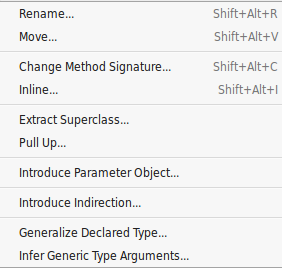
\includegraphics[scale=1]{fig-refactor-eclipse.png}
			\else
				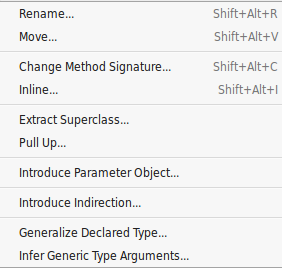
\includegraphics[scale=0.75]{fig-refactor-eclipse.png}
			\fi
			\caption{%
				Базовые методы рефакторинга реализованы в большинстве 
				современных интегрированных сред разработки, например, Eclipse
				(изображено контекстное меню этой среды для рефакторинга метода класса).}
		\end{figure}
	}

	\section{Устаревшее ПО}

	\frame{
		\frametitle{Работа с устаревшим ПО}

		\textbf{Причины использования} устаревшего ПО \engterm{legacy software}: 
		\begin{itemize}
			\item высокие затраты на разработку нового кода; 
			\item необходимость сертификации.
		\end{itemize}

		\vspace{1ex}
		\textbf{Сценарии работы} с устаревшим ПО:
		\begin{itemize}
			\item сворачивание (в случае устранения зависимостей от~системы);
			\item использование стабильной версии (система необходима, необходимость ее~модификации низка);
			\item реинженерия (качество системы снизилось из-за~внесенных изменений; необходима интеграция с~новыми компонентами);
			\item частичная или полная замена ПО (работа с~системой невозможна; оправдана разработка новой системы).
		\end{itemize}
	}

	\frame{
		\frametitle{Работа с устаревшим ПО}

		\begin{center}\small
			\begin{tabular}{|p{0.2\textwidth}|p{0.3\textwidth}|p{0.3\textwidth}|}
				\hline
				\centering Качество & \multicolumn{2}{c|}{Значимость} \cr
				\cline{2-3}
				& \centering Низкая & \centering Высокая \cr
				\hline
				Низкое & сворачивание & \raggedright реиженерия; замена, если~существует готовая походящая система \cr
				\hline
				Высокое & \raggedright использование стабильной версии; сворачивание, если~необходима значительная модификация 
					& \raggedright использование стабильной версии \cr
				\hline
			\end{tabular}
		\end{center}
	}

	\subsection{Оценка значимости системы}

	\frame{
		\frametitle{Оценка значимости системы}

		\textbf{Критерии значимости} (определяются заказчиком и конечными пользователями):
		\begin{itemize}
			\item
			интенсивность и частота использования системы;
			\item
			поддерживаемые на текущий момент производственные процессы;
			\item
			функциональная надежность системы \engterm{dependability} — корректность результатов работы системы 
			при условии наличия в ней дефектов;
			\item
			важность данных, генерируемых системой.
		\end{itemize}
	}

	\subsection{Оценка качества системы}

	\frame{
		\frametitle{Оценка качества системы}

		\textbf{Критерии качества взаимодействия с окружением:}
		\begin{itemize}
			\item
			стабильность поставщиков системы (ответственных за доставку, разворачивание и~сопровождение);
			\item
			частота отказов системы и окружения;
			\item
			возраст оборудования и ПО, стоимость их~сопровождения;
			\item
			производительность окружения;
			\item
			требования, касающиеся поддержки вспомогательного~ПО и~оборудования;
			\item
			затраты на сопровождение (напр., замену оборудования и~продление лицензий на~вспомогательное~ПО);
			\item
			интероперабельность (проблемы взаимодействия с~другим~ПО, 
			в~частности, при~сборке системы; потребность в~эмуляции оборудования).
		\end{itemize}
	}

	\frame{
		\frametitle{Оценка качества системы}

		\textbf{Критерии качества самой системы:}
		\begin{itemize}
			\item
			понятность исходного кода и дизайна;
			\item
			наличие и полнота документации;
			\item
			наличие и согласованность схемы данных;
			\item
			производительность и ее влияние на пользователей;
			\item
			используемые языки программирования;
			\item
			наличие управления конфигурацией и описания версий компонентов системы;
			\item
			наличие и полнота тестовых сценариев;
			\item
			навыки группы сопровождения.
		\end{itemize}
	}

	\section{Заключение}

	\subsection{Выводы}
	
	\frame{
		\frametitle{Выводы}

		\begin{enumerate}
			\item
			Эволюция программного обеспечения — процесс, дополняющий его~разработку. 
			В~гибкой методологии разработки эволюция производится разработчиками; 
			в~классической модели жизненного цикла эволюция может осуществляться специальной группой (\emph{сопровождение ПО}).

			\vspace{0.5ex}
			\item
			Эволюция определяется запросами на~изменение. 
			Основные фазы внедрения изменений: оценка влияния; планирование выпуска; реализация изменения.

			\vspace{0.5ex}
			\item
			Существует три типа сопровождения: исправление дефектов (в~т.\,ч.~упреждающее); 
			адаптация к~среде выполнения; внесение новой функциональности.

			\vspace{0.5ex}
			\item
			Реинженерия ПО заключается в упрощении структуры программы и / или данных и~дополнении документации. 
			Рефакторинг (внесение в программу малых изменений с~сохранением функциональности) 
			является упреждающей формой сопровождения~ПО во~время разработки.
		\end{enumerate}
	}
	
	\subsection{Материалы}
	
	\frame{
		\frametitle{Материалы}
		
		\begin{thebibliography}{9}
			\bibitem[1]{1}
			Sommerville, Ian
			\newblock Software Engineering.
			\newblock {\footnotesize Pearson, 2011. — 790 p.}

			\bibitem[2]{2}
			Fowler, Martin
			\newblock Сайт по рефакторингу.
			\newblock {\footnotesize \url{http://refactoring.com/}}

			\bibitem[3]{3}
			Лавріщева К.\,М. 
			\newblock Програмна інженерія (підручник). 
			\newblock {\footnotesize К., 2008. — 319 с.}
		\end{thebibliography}
	}
	
	\frame{
		\frametitle{}
		
		\begin{center}
			\Huge Спасибо за внимание!
		\end{center}
	}
\end{document}
